\chapter{EVALUATION}

The Information Extraction and the Ontology Similarity modules are two important part of the system.  We will evaluate them respectively.

\section{Experiments of Information Extraction }

To evaluate the performance of information extraction, we get some sentences by the sentence filters, different sentence filter can extract different kinds of sentences. We use degree sentences to explain the process:

In the experiment, we selected 100 sentences from job descriptions that are requirements of candidates degree and major. The value of degree and major are labeled manually. We use patterns to  match and extract the degree information from the sentences. The pattern is gotten from the observation of sentences. As we add more pattern, the accuracy of information increased as well. When we used 6 patterns, the accuracy of degree became 94\%. Figure \ref{fig:degree_accuracy} show the accuracy with number of patterns. The accuracies of three fields are shown in \ref{tab:ieaccura}

\begin{figure}[htbp]
  \centering
  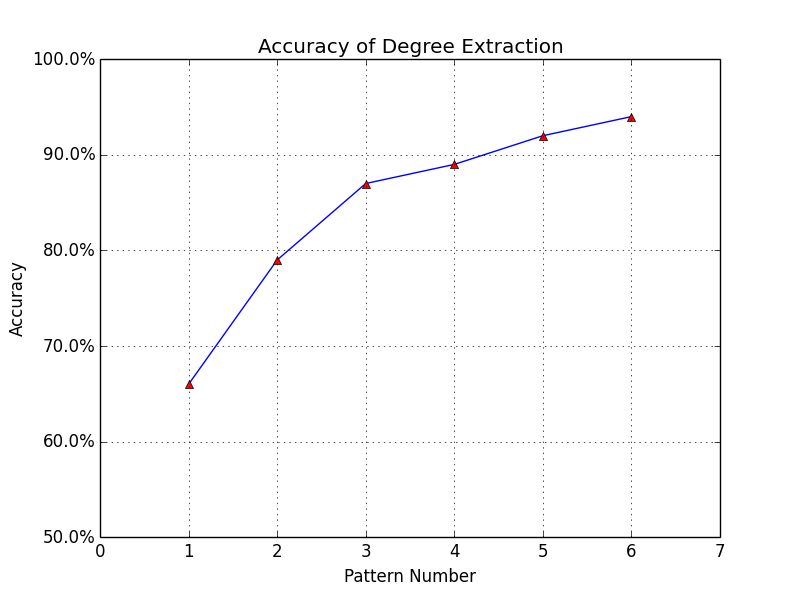
\includegraphics[scale=0.5]{images/degree_accuracy.png}
  \caption{Degree Extraction  Accuracy}
  \label{fig:degree_accuracy}
\end{figure}


\begin{table}[ht]
\caption{Information Extraction} % title of Table
\centering % used for centering table
\begin{tabular}{   | c | c | c | c |   }
 \hline
                     Field   & Pattern Num & Accuracy     \\
 \hline
                     Degree & 6         & 94\%         \\
 \hline
                     Major  & 10        & 0.85\%      \\
 \hline
                     Skill  & 6         & 0.82 \%      \\
 \hline
\end{tabular}
\label{tab:ieaccura} % is used to refer this table in the text
\end{table}

\section{Experiments of Ontology Similarity}

From the table ~\ref{tab:dismatrix2} we got similarity value between skills. There is no standard criteria to measure the similarity of two entities.  To evaluate the accuracy of our result, we compare the result with human labeled data. We tested the two data sets.



\begin{table}
\centering
\caption{ Javascript Similarity Evaluation : NDCG = 0.94 }
\begin{tabular}{ | c | c | c  | c |  }
 \hline
    Term     &  Similarity Value  &  Position   & Relevance     \\  \hline
    jQuery   &  0.1981            &      4      &   8        \\
     HTML    &  0.2087            &      3      &   4         \\
     CSS     &  0.2439            &      2      &   3   \\
     Java    &  0.0665            &      5      &   1   \\
    Python   &  0.0189            &      8      &   1   \\
     Ruby    &  0.023             &      7      &   1    \\
     JSP     &  0.0253            &      6      &   2    \\
 \hline
\end{tabular}
\label{tab:simcompare1}
\end{table}


\begin{table}
\centering
\caption{ HTML Similarity Evaluation : NDCG = 0.97 }
\begin{tabular}{ | c | c | c  | c |  }
 \hline
    Term      &  Similarity Value  &  Position   & Relevance     \\  \hline
  Javascript   &  0.2087           &      2      &   3        \\
     jQuery    &  0.0979           &      3      &   3         \\
     CSS     &  0.3569             &      1      &   5   \\
     Java    &  0.0473             &      4      &   1   \\
    Python   &  0.0175             &      6      &   1   \\
     Ruby    &  0.023              &      5      &   1    \\
     JSP     &  0.0103             &      7      &   3    \\
 \hline
\end{tabular}
\label{tab:simcompare2}
\end{table}



To evaluate the system, some measures will be used. We also proposed two evaluation method: Pre-collected Data and User's direct experience.

\section{Basic measures of the system}

In traditional information retrieval system, precision and NDCG are widely used measures ~\cite{manning2008introduction}.     Precision ($P$) is the fraction of retrieved documents that are relevant .
       $$  Precision =  \frac{ \#(releveant~items~ retrieved)}{ \#(retrieved~items)}$$
   
Since the results are ranked, $ Normalized~Discounted~Cumulative~Gain ( NDCG )$ will be an important measure to evaluate the ranked retrieval results. For a set of queries $Q$, let $R(j,d)$ be the relevance score assessors gave to document $d$ for query $j$.
       $$ NDCG(Q,k) = \frac {1}{|Q|} \sum_{j=1}^{|Q|}{Z_{kj}} \sum_{m=1}^{k} \frac{2^{R(j,m)} - 1}{ \log_2(1+m)} $$
       
where $Z_{kj}$ is a normalization factor calculated to make it so that a perfect ranking's NDCG at $k$ for query $j$ is 1. For queries for which $k' < k$ documents are retrieved, the last summation is done up to $k'$.
 

\section{Experimental Setup}

We collected some resumes from internet manually, and   job descriptions were collected by web crawler and stored in the database. In the evaluation phrase, we created a set of 100 job descriptions, which includes several kinds of jobs, like web developers, back-end developers, mobile developers and so on. The relevance value of job descriptions to each resume will be set manually. We would like to display jobs  that better match the candidate' resumes at the top. We create a query q from the resume, and treat the text of the job descriptions as documents d and apply standard ad-hoc retrieval techniques to rank the jobs.  The different retrieval algorithms we use are Okapi BM25~\cite{robertson2009probabilistic} ,   Kullback-Leibler divergence, and the TF-IDF. Since the job descriptions are fairly verbose we also experiment with a retrieval model where certain terms that are important to the quality of the match are weighted up in the TF-IDF scoring model.

\section{Experimental Results}

For our experiments to compare the various retrieval methods we used 8 candidate resumes  and retrieved the top 20 job descriptions  each method and judged the relevance of these against the resumes. The resumes we chose had an
average of 100 jobs per resume.  To compare performance of retrieval methods for the top results returned, we used
both Precision @ k e~\ref{tab:job_precision} and NDCG, shown in Table~\ref{tab:job_ndcg} . The result  shows that Ontology Similarity  performs the best. This agrees with results in  where it was found that finding and weighting
up important concepts in long queries can improve retrieval performance.

\begin{table}[ht]
\caption{Precision of Job Ranking } % title of Table
\centering % used for centering table
\begin{tabular}{    | c | c | c | c | c |  }
 \hline
       k     & Okapi BM25 & KL    & TF-IDF & Ontology Similarity  \\
 \hline
       5     & 0.13       & 0.40  & 0.54     & 0.74   \\
 \hline
       10    & 0.16       & 0.36  & 0.50     & 0.66   \\
 \hline
       20    & 0.16       & 0.35  & 0.49     & 0.61   \\
 \hline

\end{tabular}
\label{tab:job_precision} % is used to refer this table in the text
\end{table}


\begin{table}[ht]
\caption{NDCG of Job Ranking } % title of Table
\centering % used for centering table
\begin{tabular}{    | c | c | c | c | c |  }
 \hline
       k    & Okapi BM25 & KL    & TF-IDF & Ontology Similarity  \\
 \hline
       5    & 0.15       & 0.34  & 0.45     & 0.78   \\
 \hline
       10   & 0.18       & 0.44  & 0.47     & 0.72   \\
 \hline
       20   & 0.19       & 0.35  & 0.45     & 0.66   \\
 \hline
 
\end{tabular}
\label{tab:job_ndcg} % is used to refer this table in the text
\end{table}



